\documentclass[a4paper, 11pt, twoside]{article}

\usepackage{hyperref}
%\usepackage[ngerman]{babel}
\usepackage[english]{babel}
%\usepackage[latin1]{inputenc}
\usepackage[utf8]{inputenc}

\usepackage{graphicx,float,subfigure}
%\usepackage{pifont}
\usepackage{type1cm}
\usepackage{amssymb, amsthm, amsmath}
\usepackage{listings}
\usepackage{transparent}
\usepackage[usenames,dvipsnames]{color}

\setcounter{tocdepth}{5}
\setcounter{secnumdepth}{5}


\usepackage[ampersand]{easylist}


%%% For Code

\usepackage{color}
\definecolor{gray}{rgb}{0.4,0.4,0.4}
\definecolor{darkblue}{rgb}{0.0,0.0,0.6}
\definecolor{cyan}{rgb}{0.0,0.6,0.6}


%%% Define Language

\lstset{
  basicstyle        = {\footnotesize\ttfamily},
  breaklines        = true,
  tabsize           = 4,
  columns           = fullflexible,
  showstringspaces  = false,
  %showspaces        = true,
  commentstyle      = \color{gray}\upshape
}

\lstdefinelanguage{XML}
{
  frame 		      = single,
  morestring          = [b]",
  morestring          = [s]{>}{<},
  morecomment         = [s]{<?}{?>},
  morecomment         = [s]{!--}{--},
  commentstyle        = \color{OliveGreen}\upshape,
  stringstyle         = \color{black},
  identifierstyle     = \color{NavyBlue},
  keywordstyle        = \color{NavyBlue},
  morekeywords        = {xmlns,version,type}% list your attributes here
}


\lstdefinelanguage{CustomC++}
{
  language        = C++,
  frame 		  = single,
  keywordstyle    = \color{NavyBlue}, 
  numbers         = none,
  commentstyle    = \color{OliveGreen}\upshape,
  stringstyle     = \color{Orchid},
}







%%% Environments for Theorems, Definitions...

\theoremstyle{plain}
\newtheorem{thm}{Theorem}
\newtheorem*{Co}{Cosserat's Theorem}
\theoremstyle{definition}
\newtheorem*{Weak}{Weak Formulation}







\usepackage{pgf}
\usepackage{url}
%\usepackage{graphicx}
%\usepackage{pifont}
%\usepackage{type1cm}


\providecommand{\abs}[1]{\lvert#1\rvert}
\providecommand{\norm}[1]{\lVert#1\rVert}


\DeclareMathOperator\tr{tr}
\DeclareMathOperator\diam{diam}
\DeclareMathOperator\Div{div}

\newcommand{\dd}{\,\mathrm{d}}
\newcommand{\R}{\mathbb{R}}






\usepackage{makeidx}

\makeindex

\setlength{\parindent}{0em}
\setlength{\oddsidemargin}{0.0cm}
\setlength{\evensidemargin}{0.0cm}
\setlength{\textheight}{23cm}
\setlength{\topmargin}{-0.5cm}
\setlength{\footskip}{1.5cm}
\setlength{\textwidth}{15.5cm}

\renewcommand*\familydefault{\sfdefault}






\begin{document}


\thispagestyle{empty}

%\documentclass[a4paper]{article}

%\usepackage{pgf}
%\usepackage{graphicx}
%\usepackage{pifont}
%\usepackage{type1cm}

\setlength{\textwidth}{14cm}
\setlength{\oddsidemargin}{1cm}

%\begin{document}

\thispagestyle{empty}

%%%%%%%%%%%%%%%%%%%%%%%%%%%%%%%%%%%%%%%%
%%%%%%%%%%%%%%%%%%%%%%%%%%%%%%%%%%%%%%%%
%%%%%%%%%%%%%%%%%%%%%%%%%%%%%%%%%%%%%%%%

\newcount \Z
\Z=20

%%% logos %%%

%%% NUMHPC %%%
\newlength{\numhpclogox}
\setlength{\numhpclogox}{\paperwidth} % 20/210ths of the paperwidth
\divide\numhpclogox by 210
\multiply\numhpclogox by 100

\newlength{\numhpclogoy}
\setlength{\numhpclogoy}{\paperheight} % 270/297ths of the paperwidth
\divide \numhpclogoy by 297
\multiply \numhpclogoy by -235

\newlength{\numhpclogoheight}
\setlength{\numhpclogoheight}{\paperheight} % 270/297ths of the paperwidth
\divide\numhpclogoheight by 297
\multiply\numhpclogoheight by 20

%%% KIT %%%
\newlength{\kitlogox}
\setlength{\kitlogox}{\paperwidth} % 20/210ths of the paperwidth
\divide\kitlogox by 210
\multiply\kitlogox by 0

\newlength{\kitlogoy}
\setlength{\kitlogoy}{\paperheight} % 270/297ths of the paperwidth
\divide \kitlogoy by 297
\multiply \kitlogoy by -230

\newlength{\kitlogoheight}
\setlength{\kitlogoheight}{\paperheight} % 270/297ths of the paperwidth
\divide\kitlogoheight by 297
\multiply\kitlogoheight by 15


%%% EMCL %%%
\newlength{\emcllogox}
\setlength{\emcllogox}{\paperwidth} % 20/210ths of the paperwidth
\divide\emcllogox by 210
\multiply\emcllogox by 28

\newlength{\emcllogoy}
\setlength{\emcllogoy}{\paperheight} % 270/297ths of the paperwidth
\divide \emcllogoy by 297
\multiply \emcllogoy by -160

\newlength{\emcllogoheight}
\setlength{\emcllogoheight}{\paperheight} % 270/297ths of the paperwidth
\divide\emcllogoheight by 297
\multiply\emcllogoheight by 20

%%% HIFLOW %%%
\newlength{\hiflowlogox}
\setlength{\hiflowlogox}{\paperwidth} % 20/210ths of the paperwidth
\divide\hiflowlogox by 210
\multiply\hiflowlogox by 28

\newlength{\hiflowlogoy}
\setlength{\hiflowlogoy}{\paperheight} % 270/297ths of the paperwidth
\divide \hiflowlogoy by 297
\multiply \hiflowlogoy by -160

\newlength{\hiflowlogoheight}
\setlength{\hiflowlogoheight}{\paperheight} % 270/297ths of the paperwidth
\divide\hiflowlogoheight by 297
\multiply\hiflowlogoheight by 33

%%%%%%%%%%%%%%%%%%%%%%%%%%%%%%%%%%%%%%%%
%%%%%%%%%%%%%%%%%%%%%%%%%%%%%%%%%%%%%%%%
%%%%%%%%%%%%%%%%%%%%%%%%%%%%%%%%%%%%%%%%

%%% NUMHPC %%%
%%\pgftext[bottom, left, at={\pgfpointadd{\pgfpoint{0pt}{0pt}}{\pgfpoint{\numhpclogox}{\numhpclogoy}}}]{\includegraphics[totalheight=\numhpclogoheight]{numhpc}}

%%% KIT %%%
%%\pgftext[bottom, left, at={\pgfpointadd{\pgfpoint{0pt}{0pt}}{\pgfpoint{\kitlogox}{\kitlogoy}}}]{\includegraphics[totalheight=\kitlogoheight]{kitlogo}}

%%% EMCL %%%
\pgftext[bottom, left, at={\pgfpointadd{\pgfpoint{0pt}{0pt}}{\pgfpoint{\hiflowlogox}{\hiflowlogoy}}}]{
\includegraphics[totalheight=\hiflowlogoheight]{HF3_color}}

%%% horizontal lines %%%
\pgfline{\pgfxy(-1pt,0.1pt)}{\pgfxy(15pt,0.1pt)}
\pgfline{\pgfxy(-1pt,-21.4pt)}{\pgfxy(15pt,-21.4pt)}
%%\pgfline{\pgfxy(-1pt,-22.4pt)}{\pgfxy(15pt,-22.4pt)}

%%% EMCL text %%%
\pgftext[bottom, left, at={\pgfpointadd{\pgfpoint{0pt}{0pt}}{\pgfpoint{0cm}{1cm}}}]{{\LARGE{{\bf Tutorial}}}}

%%% EMCL web %%%
\pgftext[bottom, left, at={\pgfpointadd{\pgfpoint{0pt}{0pt}}{\pgfpoint{10.5cm}{-21.7cm}}}]{{\fontsize{13}{10}\selectfont{} http://www.hiflow3.org/}}

\hspace{2cm}
\begin{picture}(0,0)(-250,-25)

\includegraphics[scale=.22]{emcl.pdf} 
\end{picture}

%%% author %%%
\pgftext[bottom, left, at={\pgfpointadd{\pgfpoint{0pt}{0pt}}{\pgfpoint{0cm}{-4cm}}}]{{
\begin{parbox}{13cm}{
\begin{center}\fontsize{12}{30}\selectfont{} Nicolai Schoch, Fabian Kißler
\end{center}}
\end{parbox}}}

%%% title %%%
\pgftext[bottom, left, at={\pgfpointadd{\pgfpoint{0pt}{0pt}}{\pgfpoint{0cm}{-7.5cm}}}]{{
\begin{parbox}{13cm}{
%%\begin{center}\fontsize{18}{30}\selectfont{} \bf Using HiFlow$^3$ for solving the
\begin{center}\fontsize{22}{30}\selectfont{} \bf Elasticity Tutorial \\ for Soft Tissue Simulation
\end{center}}
\end{parbox}}}

%%% date %%%
\pgftext[bottom, left, at={\pgfpointadd{\pgfpoint{0pt}{0pt}}{\pgfpoint{0cm}{-16.4cm}}}]{{
\begin{parbox}{13cm}{
\begin{center}\fontsize{12}{24}\selectfont{} 
\vspace{5cm}
\textit{modified on \today}\\ 
\vspace{6.5cm}
\hspace{6cm}\textit{Version 1.5}
\end{center}}
\end{parbox}}}

%fhfh \hfill sjdh

%\end{document}


%\newpage
%\null\newpage




\newtheorem{remark}{Remark}[section]
\thispagestyle{empty}
\tableofcontents





\newpage
\pagestyle{plain}
\framebox[15.5cm]{\parbox[c][2.3cm]{14.0cm}{
{\fontsize{19}{30}\selectfont{} \bf{Applying HiFlow$^3$ for solving an \\ Elasticity Problem for Soft Tissue Simulation}
}}}
\vspace{0.5cm}
\section{Introduction}

HiFlow$^3$ is a multi-purpose finite element software providing powerful tools for efficient and accurate solution to a wide range of problems modeled by partial differential equations (PDEs). Based on object-oriented concepts and the full capabilities of C++ the HiFlow$^3$ project follows a modular and generic approach for building efficient parallel numerical solvers. It provides highly capable modules dealing with the mesh setup, finite element spaces, degrees of freedom, linear algebra routines, numerical solvers, and output data for visualization. Parallelism - as the basis for high performance simulations on modern computing systems - is introduced on two levels: coarse-grained parallelism by means of distributed grids and distributed data structures, and fine-grained parallelism by means of platform-optimized linear algebra back-ends.





\subsection{How to Use the Tutorial?}

You find the example code (elasticity\_tutorial.cc, elasticity\_tutorial.h) and a parameter file for the first numerical example (elasticity\_tutorial.xml) in the folder \verb'/hiflow/examples/elasticity'. The geometry data (stanford\_bunny.inp) is stored in the folder \\ \verb'/hiflow/examples/elasticity/SimInput'.



\subsubsection{Using HiFlow$^3$ as a Developer}\label{sectiondeveloper}


First build and compile HiFlow$^3$. 
Go to the directory \verb'/build/example/elasticity', where the binary \texttt{elasticity\_tutorial} is stored. 
Type
\begin{lstlisting}[breaklines]
  ./elasticity_tutorial /"path_to"/elasticity_tutorial.xml
\end{lstlisting}
to execute the program in sequential mode. 
To execute in parallel mode \index{program!executing in parallel} with \verb'X' processes, type
\begin{lstlisting}[breaklines]
  mpirun -np X elasticity_tutorial /"path_to"/elasticity_tutorial.xml
\end{lstlisting}
In both cases, you need to make sure that the default parameter file \verb'elasticity_tutorial.xml' is stored in the same directory as the binary, and that the geometry data specified in the parameter file is stored in \verb'/hiflow/examples/data'. 
Alternatively, you can specify the path of your own xml-file, i.e.
\begin{lstlisting}[breaklines]
  ./elasticity_tutorial /"path_to_parameter_file"/"name_of_parameter_file".xml
\end{lstlisting}







\section{Mathematical Setup}

\subsection{Problem}
\label{ssec:problem_description}

We want to investigate the deformation of an elastic solid subject to external forces.
In the following, the solid will be represented by a bounded subset $\Omega \subset \mathbb{R}^3$.
The Cauchy stress tensor and the infinitesimal strain tensor will be denoted by $\sigma$ and $\epsilon$, respectively.
Given any point $p \in \Omega$ and any surface passing through $p$, let $n$ denote a unit normal vector to this surface at $p$.
Then, the stress vector at $p$ w.r.t. $n$ is given by
\begin{equation}
 T^{(n)} = n \sigma.
\end{equation}
According to this formula, the computation of the stress vector does not depend on the choice of the surface passing through $p$.
If we apply pressure to the surface of the solid, that is, given any surface force density $g = n \sigma^\partial$, we have
\begin{equation}
 g = n \sigma
\end{equation}
on the boundary $\partial \Omega$ with unit normal vector field $n$.
Generally, pressure will only act on a certain subset of $\partial\Omega$, the effective Neumann boundary $\Gamma_{\text{N}}^{\neq 0}$.
Furthermore, there is a Dirichlet boundary $\Gamma_{\text{D}}$ with $\Gamma_{\text{D}} \cap \Gamma_{\text{N}}^{\neq 0} = \emptyset$.
Let $u$ be the displacement vector field associated to the deformation, that is, for any $p \in\Omega$,
\begin{equation}
	p' = p + u(p)
\end{equation}
represents the position of the particle $p$ after the deformation.
By $u^\partial$ we denote a given displacement on the Dirichlet boundary.
We define the Neumann boundary $\Gamma_{\text{N}} := \partial\Omega \setminus \Gamma_{\text{D}}$ with $g = 0$ on $\Gamma_{\text{N}} \setminus \Gamma_{\text{N}}^{\neq 0}$ (for illustration, see figure \ref{fig:liver}).

\begin{figure}[htb]
	\centering 
	\def\svgwidth{200pt} 
	\input{liver.pdf_tex}
	\caption{Partition of the boundary of $\Omega$: The red line represents the Dirichlet boundary. The remaining part is the Neumann boundary with the effective Neumann boundary, represented by the blue line, as a subset.} 
	\label{fig:liver}
\end{figure}

The infinitesimal strain tensor $\epsilon$ relates the deformation gradient $\nabla u$ to the deformation $u$ of $\Omega$.
If we assume that the displacement gradients are small compared to the diameter of $\Omega$, we have
\begin{equation}
 \epsilon(u) = \frac{1}{2} \left( \nabla u + \nabla u ^ T \right). 
\end{equation}
Note that the infinitesimal strain tensor is the linearized version of the finite strain tensor.
Furthermore, we require Hooke's Law to hold, or, to put it in another way, we want that there is a linear relation between the Cauchy stress tensor and the infinitesimal strain tensor.
If $C$ denotes the fourth-order stiffness tensor, using Einstein summation, we get
\begin{equation}
 \sigma_{ij} = C_{ijkl} \epsilon_{kl}.
\end{equation}
When using Voigt notation, we obtain
\begin{equation}
 \sigma = \lambda \tr(\epsilon) I + 2 \mu \epsilon, 
 \label{eq:CauchyStressLinear}
\end{equation}
for homogeneous and isotropic materials, where $\lambda$ and $\mu$ are Lam\'{e}'s parameters.
Note that other types of engineering constants such as Poisson's ratio $\nu$ and Young's modulus $E$ can be expressed in terms of Lam\'{e}'s parameters and vice versa:
\begin{align*}
 \nu &= \frac{\lambda}{2(\lambda + \mu)}  & E &= \frac{\mu (3 \lambda + 2 \mu)}{\lambda + \mu}  \\
 \lambda &= \frac{E \nu}{(1+\nu)(1-2\nu)} & \mu &= \frac{E}{2(1+\nu)} 
\end{align*}
Enforcing physical reality, we require $\mu,\lambda > 0$.
In terms of $E$ and $\nu$ we have $E > 0$ and $0 < \nu < 0.5$.
For more details we refer to \cite{braess} or \cite{rannacher}.
As mentioned before, deformation of the solid can be caused by forces acting on its surface.
However, we also want to consider forces acting on all the particles, e.g. gravity, which are represented by the body force density $f$.
%Assuming that the mass of the solid and momentum are conserved throughout the process of deformation, it is necessary that
Assuming that the body $\Omega$ is in a state of equilibrium, all forces and momentums acting on the surface and volume of an arbitrary subset $V \subseteq \Omega$ add up to zero:
\begin{align}
 0 &= \underbrace{\int_{V} f(x) \dd x}_{\text{body force}}  + \underbrace{\int_{\partial V} \sigma(x) n \dd S}_{\text{surface force}}. \\
 \intertext{Using the divergence theorem, we get}
 0 &= \int_{V} f(x) + \Div(\sigma(x)) \dd x ,
\end{align}
which, since $V$ is an arbitrary subset and $f$ and $\Div \sigma$ are supposed to be continuous functions, yields the differential equation
\begin{equation}
 -\Div\sigma = f.
 \label{eq:elasticityPDE}
\end{equation}
A detailed derivation of equation \eqref{eq:elasticityPDE} can be found in \cite{braess}.
Furthermore, we require the stiffness tensor to be symmetric, positive definite on symmetric dyads and sufficiently smooth:
\begin{equation}
 C_{ijkl} \in C^2 (\overline{\Omega}), \quad C_{ijkl} = C_{klij}, \quad C_{ijkl}\epsilon_{ij}\epsilon_{kl} > 0, \text{ if }  \epsilon \neq 0.
\end{equation}
All things considered, assuming that $f$, $\sigma^\partial$ and $u^\partial$ are sufficiently smooth, we need to find functions $u$, $\epsilon$ and $\sigma$, whose components need to satisfy the following regularity conditions
\begin{equation}
 u_i \in C(\Omega \cup \Gamma_\text{D}) \cap C^1(\Omega), \quad
 \epsilon_{ij} \in C(\Omega) \cap L^2(\Omega), \quad
 \sigma_{ij} \in C(\Omega \cup \Gamma_\text{N}) \cap C^1(\Omega) \cap L^2(\Omega)
\end{equation}
and the equilibrium equations of linear elasticity:
\begin{center}\framebox[6.0cm]{\parbox[c][3.5cm]{15.5cm}{
{ \begin{alignat}{2}
 -\Div \sigma &= f &\quad& \text{ on }\Omega, \label{eq:elasticity} \\
 u        &= u^\partial && \text{ on }\Gamma_\text{D}, \\
 n \sigma &= g && \text{ on }\Gamma_\text{N}, \\
 \frac{1}{2} \left( \nabla u + \nabla u ^ T \right) &= \epsilon && \text{ on }\Omega, \\
 \sigma   &= C\epsilon && \text{ on }\Omega.
\end{alignat}
}}}\end{center}
Since the existence of a classical solution to this problem cannot be guaranteed, we will derive the so-called weak formulation of the problem in the succeeding section. 
However, the following theorem by Cosserat states that the difference of two solutions describes the motion of a rigid body and gives a uniqueness criterion based on the geometry of $\Omega$.
\begin{Co}
Let $u^{(1)}$ and $u^{(2)}$ denote two classical solutions to the foregoing system of partial differential equations.
Then there is a vector $b \in \R^3$ and a skew symmetric matrix $B \in \R^{3 \times 3}$ such that 
\begin{equation}
	u^{(1)}(x) - u^{(2)}(x) = b + B x
\end{equation}
for all $x \in \Omega$.
Additionally, if $\Gamma_{\text{D}}$ contains three linearly independent vectors, we have $b=0$ and $B=0$ and the solution to the equilibrium equations of linear elasticity is unique.
\end{Co}














\subsection{Weak Formulation}

We begin by introducing some notation and basic definitions.
Let $L^2(\Omega)$ denote the set of square integrable functions on $\Omega$ with the following inner product and norm:
\begin{equation}
	(f,g)_\Omega = \int_\Omega f g \dd x , \quad
	\norm{f}_\Omega = \sqrt{ \int_\Omega \abs{f}^2 \dd x }.
\end{equation}
The Sobolev space $H^1(\Omega)$ is the completion of $C^\infty(\overline{\Omega})$ with respect to the norm given by
\begin{equation}
	\norm{f}_{1;\Omega} = \sqrt{ \norm{f}_\Omega^2 + \int_\Omega \abs{\nabla f}^2 \dd x },
\end{equation}
and let $H^1_0(\Gamma_\text{D};\Omega)$ be the closure of the subset
\begin{equation}
	\{ f \in C^\infty(\overline{\Omega}) : f = 0  \text{ on } \Gamma_{\text{D}} \} \subseteq H^1(\Omega).
\end{equation}

Moreover, in order to ensure that the following propositions and declarations are well-defined, we need the statements (A1) to (A4) to hold:
\begin{itemize}
	\item[(A1)] The subset $\Omega \subset \R^3$ satisfies the strong cone condition.
	\item[(A2)] The measure of $\Gamma_{\text{D}} \subset \partial\Omega$ is positive and its relative interior contains three linearly independent vectors.
	\item[(A3)] On $\Omega$, the stiffness tensor $C = (C_{ijkl})$ is symmetric and uniformly bounded,
	\begin{equation}
		C_{ijkl} = C_{klij} \in L^{\infty}(\Omega),
	\end{equation}
	as well as positive definite, i.e.,
	\begin{equation}
		C_{ijkl}\epsilon_{ij}\epsilon_{kl} > 0
	\end{equation}
	for all symmetric tensors $\epsilon \neq 0$.
	\item[(A4)] The external forces acting on the solid and the displacement of the boundary are given by 
	\begin{equation}
		f \in L^2(\Omega)^3, \quad \sigma^\partial \in H^1(\partial\Omega)^{3 \times 3}_{\text{sym}}, \quad u^\partial \in H^1(\Omega)^3.
	\end{equation}
\end{itemize}



Now, we can derive the weak formulation of the equilibrium equations of linear elasticity.
Using previous notation, we multiply equation \eqref{eq:elasticity} by an arbitrary test function $v \in  C^\infty (\Omega)^3$ and integrate over $\Omega$.
This yields
\begin{equation}
 - \int_\Omega \Div(\sigma(u)) v \dd V = \int_\Omega f v \dd V .
 \label{eq:WeakFormulation}
\end{equation}
Integrating the left hand side by parts gives
\begin{equation}
 - \int_{\partial\Omega} \sigma(u) v \dd \vec{S} + \int_\Omega \sigma_{ij} \partial_i v_j \dd V = \int_\Omega f v \dd V .
 \label{eq:WeakIntegrationByParts}
\end{equation}
Note that the Cauchy stress tensor $\sigma(u)$, given by equation \eqref{eq:CauchyStressLinear}, is symmetric.
Hence, we can rewrite the second term on the left hand side of equation \eqref{eq:WeakIntegrationByParts}:
\begin{align}
 \int_\Omega \sigma_{ij} \partial_i v_j \dd V &= \frac{1}{2} \int_\Omega \sigma_{ij} \partial_i v_j + \sigma_{ji} \partial_i v_j \dd V \\
 &= \int_\Omega \sigma_{ij} \left( \frac{1}{2} \left( \partial_i v_j + \partial_j v_i \right) \right) \dd V \\
 &= \int_\Omega \sigma(u) : \epsilon(v) \dd V,
\end{align}
which denotes the Frobenius inner product, where $A:B = A_{ij} B_{ij}$.
We hence obtain
\begin{equation}
  \int_\Omega \sigma(u) : \epsilon(v) \dd V = \int_\Omega f v \dd V + \int_{\partial\Omega} \sigma(u) v \dd \vec{S}.
  \label{eq:WeakNearlyFinal}
\end{equation}
We can rewrite the second summand on the right-hand side in terms of the surface force density $g$ by using the fact that $\partial\Omega$ is the disjoint union of $\Gamma_\text{D}$ and $\Gamma_\text{N}$:
\begin{align}
 \int_{\partial\Omega} \sigma(u) v \dd \vec{S} &= \int_{\partial\Omega} n \sigma(u) v \dd S \\
 &= \int_{\Gamma_\text{D}} n \sigma(u) v \dd S + \int_{\Gamma_\text{N}} g v \dd S.
\end{align}
All things considered, we get
\begin{equation}
  \int_\Omega \sigma(u) : \epsilon(v) \dd V = \int_\Omega f v \dd V + \int_{\Gamma_\text{D}} n \sigma(u) v \dd S + \int_{\Gamma_\text{N}} g v \dd S.
  \label{eq:WeakFinal}
\end{equation}
In order to shorten notation, we define the bilinear form $a$ and the linear form $l$:
\begin{equation}
	a(u,v) := \int_\Omega \sigma(u) : \epsilon(v) \dd V, \quad
	l(v) := \int_\Omega f v \dd V + \int_{\Gamma_\text{N}} g v \dd S
\end{equation}
Note that in the definition of $l$ we omitted the second term on the right-hand side of equation \eqref{eq:WeakFinal}, as if we considered homogeneous Dirichlet boundary conditions, i.e. $u^\partial = 0$ on $\Gamma_\text{D}$.
We will correct this error by requiring the difference $u-u^\partial$ of the solution $u$ and the given translation vector field $u^\partial$ to vanish on the boundary $\Gamma_\text{D}$, i.e. $u-u^\partial \in H_0^1(\Gamma_\text{D};\Omega)^3$.
You will find the same method being used in the implementation below, where the Dirichlet boundary conditions are considered separately in the assembly of the system, see \ref{sssec:assemble_system}.
%%%finding a solution $u \in H^1(\Omega)^3$ such that the difference $u-u^\partial$ vanishes on $\Gamma_\text{D}$, i.e. $u-u^\partial \in H_0^1(\Gamma_\text{D};\Omega)^3$.
%%% altering the solution space:
%%% We want to find a solution $u \in H^1(\Omega)^3$ such that $u-u^\partial \in H_0^1(\Gamma_\text{D};\Omega)^3$.
The weak formulation of the equilibrium equations of linear elasticity now reads as follows:
\begin{center}\framebox[10.5cm]{\parbox[c][2.0cm]{15.5cm}{
{ \begin{center}
Find $u \in H^1(\Omega)^3$ such that $u-u^\partial \in H_0^1(\Gamma_\text{D};\Omega)^3$ and
\begin{equation}
	a(u,\varphi) = l(\varphi) \quad \forall \varphi\in H_0^1(\Gamma_\text{D};\Omega)^3.
\end{equation}
\end{center}
}}}\end{center}
As stated in Theorem 1.10 in \cite{rannacher}, assuming (A1) to (A4) hold, there is a unique weak solution to the equilibrium equations of linear elasticity.
According to the derivation of the weak formulation of the problem, every classical solution is also a weak solution and vice versa, if the weak solution satisfies the necessary regularity conditions.

One can directly recognize the terms of the above weak formulation in the implementation, see sections \ref{ssec:Member_Functions} and \ref{ssec:Assembly_Functions}.
Please note that our above derivation represents the stationary consideration of an elastic deformation process. 
In order to describe an instationary simulation, we would need to consider additional terms accounting for inertia and damping. 
This results in a more complicated assembly, and can best be solved using e.g. the Newmark time integration scheme, which guarantees for stable and efficient simulation results, see \cite{bathe}.





\section{The Commented Program}

\subsection{Preliminaries}

HiFlow$^3$ is designed for high performance computing on massively parallel machines. 
So it applies the Message Passing Interface (MPI)\index{Message Passing Interface (MPI)}\index{MPI} library specification for message-passing, see sections \ref{ssec:main} and \ref{sssec:run}, as well as \cite{MPI} and \cite{MPIstandard} .
The elasticity tutorial needs the following two input files:
\begin{itemize}
\item A parameter file: 
The parameter file is an xml-file, which contains all parameters needed to execute the program. 
It is read in by the program. 
It is not necessary to recompile the program, when parameters in the xml-file are changed. 
By default the elasticity tutorial reads in the parameter file \texttt{elasticity\_tutorial.xml}, see section \ref{sec:parameter_file}, which contains the parameters of the included example, see section \ref{sec:example}.
This file is stored in \verb'/hiflow/examples/elasticity/'.  

\item Geometry data\index{geometry data}: 
The file containing the geometry is specified in the parameter file. 
In the example in section \ref{sec:example} we used \verb'stanford_bunny.inp'.
\end{itemize}
HiFlow$^3$ does not generate meshes\index{mesh!generate} for the domain $\Omega$.\index{domain geometry!generating} Meshes in *.inp and *.vtu format can be read in. 
It is possible to extend the reader for other formats.
Furthermore, it is possible to generate other geometries by using external programs (Mesh generators) or by hand.






%%% Eingabedaten


\subsection{Parameter File}
\index{parameter file}
\label{sec:parameter_file}

The needed parameters are initialized in the parameter file \verb'elasticity_tutorial.xml'.

\lstinputlisting[language=XML]{Code/elasticity_Bunny_Scenario_DirBC.xml}

Since, for reasons of simplicity and better understandability, we do not consider effective (i.e. non-zero) Neumann force or pressure boundary conditions in the tutorial, this part is not included in the sample parameter file either.
However, we want to shortly outline the integration of Neumann boundary conditions here:
First of all, one has to declare an effective Neumann boundary $\Gamma_\text{N}^{\neq 0}$. 
This can be done by simply including an additional line \verb'<NeumannMaterialX>' in the \verb'<Boundary>' part of the parameter file. 
An additional Neumann boundary assembler class similar to the class \verb'StationaryElasticityAssembler' in \ref{sssec:StationaryElasticityAssembler} must loop over all these Neumann boundary elements and compute the effective force or pressure. 
Creating an object of the Neumann boundary class in \ref{sssec:assemble_system} then allows for integrating it according to the weak formulation.





%%% Struktur des Programms


\subsection{Structure of the Elasticity Tutorial}

Following member functions are defined in the class \verb'Elasticity'.
The survey reflects the access relations between the functions, classes and structures. 
 \begin{itemize}
    \item run()
    \begin{itemize}
		\item setup\_linear\_algebra()
		\item read\_mesh()
		\item prepare()
    \begin{itemize}
      \item prepare\_bc\_stationary()
      \begin{itemize}
        \item StationaryElasticityAssembler\_DirichletBC\_3D
      \end{itemize}
    \end{itemize}
		\item assemble\_system()
    \begin{itemize}
		\setlength{\itemindent}{18px}
        \item[$\cdot$] StationaryElasticityAssembler
    \end{itemize}
		\item solve\_system()
		\item visualize()
    \end{itemize}
 \end{itemize} 
You can find the source code of every member function in an extra section below. 







%%% main()

\subsection{Main Function}
\index{MPI}
\label{ssec:main}

The main function starts the simulation of the elasticity problem (\verb'elasticity_tutorial.cc').

\lstinputlisting[language=CustomC++]{Code/elasticity_main.cc}


%%% run()

\subsection{Member Functions}
\label{ssec:Member_Functions}

\subsubsection{run()}
\label{sssec:run}

The member function \verb'run()' is defined in the class \verb'Elasticity' (\verb'elasticity_tutorial.cc').

\lstinputlisting[language=CustomC++]{Code/elasticity_run.cc}




%%% setup\_linear\_algebra()

\subsubsection{setup\_linear\_algebra()}

The method \verb'setup_linear_algebra()' reads in the needed parameters \verb'Platform', \verb'Implementation', \verb'MatrixFormat' and \verb'PreconditionerName' from the parameter file \ref{sec:parameter_file}.

\lstinputlisting[language=CustomC++]{Code/elasticity_setup_linear_algebra.cc}


%%% read\_mesh

\subsubsection{read\_mesh()}
\label{sssec:read_mesh}

The member function \verb'read_mesh()' reads in the initial mesh, partitions, distributes and writes out the mesh.

\lstinputlisting[language=CustomC++]{Code/elasticity_read_mesh.cc}


%%% prepare

\subsubsection{prepare()}

The member function \verb'prepare()' reads in parameters regarding the physical properties of the body like \verb'density', \verb'mu', \verb'lambda' and \verb'gravity', see the remark about Lam\'{e}'s parameters in section \ref{ssec:problem_description} for details.
Furthermore, we initialize the FE space, the system matrix, the solution and right-hand side vector and execute the setup of the linear solver and preconditioner.
Since we solve the stationary elasticity problem, the function calls \verb'prepare_bc_stationary()', see \ref{para:prepare_bc_stationary}.

\lstinputlisting[language=CustomC++]{Code/elasticity_prepare.cc}


%%%%%% prepare\_bc\_stationary()

\paragraph{prepare\_bc\_stationary()}
\label{para:prepare_bc_stationary}

The \verb'Boundary' parameters in the parameter file determine whether a point will be shifted.
We create a \verb'StationaryElasticityAssembler_DirichletBC_3D' object, see section \ref{sssec:StationaryElasticityAssemblerDirichletBC3D}.

\lstinputlisting[language=CustomC++]{Code/elasticity_prepare_bc_stationary.cc}


%%% assemble\_system

\subsubsection{assemble\_system()}
\label{sssec:assemble_system}

In the member function \verb'assemble_system()', we create the \verb'StationaryElasticityAssembler' object \verb'local_asm', see section \ref{sssec:StationaryElasticityAssembler}, and call methods for the assembly of the system matrix and the right-hand side vector.
In case an effective non-zero Neumann boundary condition should be considered, this is the above mentioned place to do so, too.

\lstinputlisting[language=CustomC++]{Code/elasticity_assemble_system.cc}


%%% solve\_system

\subsubsection{solve\_system()}

After the setup of the system matrix, solution and right-hand side vector is done, we can compute the solution.

\lstinputlisting[language=CustomC++]{Code/elasticity_solve_system.cc}


%%% visualize

\subsubsection{visualize()}

The member function \verb'visualize()' writes out data for visualization.

\lstinputlisting[language=CustomC++]{Code/elasticity_visualize.cc}


\subsection{Assembly Functions}
\label{ssec:Assembly_Functions}

%%%%%%%%% StationaryElasticityAssembler\_DirichletBC\_3D

\subsubsection{StationaryElasticityAssembler\_DirichletBC\_3D}
\label{sssec:StationaryElasticityAssemblerDirichletBC3D}

In \ref{para:prepare_bc_stationary} we create an object of the structure \verb'StationaryElasticityAssembler_DirichletBC_3D', which is part of the header file \verb'elasticity_tutorial.h'.
This structure realizes the Dirichlet boundary conditions, i.e. the displacement of the points.
In the example in section \ref{sec:example}, we modify the Dirichlet boundary conditions and the respective output.


\lstinputlisting[language=CustomC++]{Code/elasticity_StationaryElasticityAssembler_DirichletBC_3D.h}



%%%%%% prepare\_bc\_stationary()

\subsubsection{StationaryElasticityAssembler}
\label{sssec:StationaryElasticityAssembler}

This class implements the system matrix and right-hand side vector locally for each cell. 
It can be found in \verb'elasticity_tutorial.h'.
We create an object of this class in \ref{sssec:assemble_system}.

\lstinputlisting[language=CustomC++]{Code/elasticity_StationaryElasticityAssembler.h}














%%%% Program Output



\section{Program Output and Visualization}
HiFlow$^3$ can be executed in a parallel or sequential mode which influences the generated output data. 
Note that the log files can be viewed by any editor.
Executing the program in parallel mode with \verb'X' processes by
\begin{lstlisting}[breaklines]
  mpirun -np X elasticity_tutorial /"path_to"/elasticity_tutorial.xml
\end{lstlisting}
or in sequential mode by
\begin{lstlisting}[breaklines]
  ./elasticity_tutorial /"path_to"/elasticity_tutorial.xml
\end{lstlisting}
generates following output data.
\begin{itemize}
  \item Mesh/geometry data:
    \begin{itemize}
      \item \texttt{elasticity\_tutorial\_initial\_mesh\_local.pvtu} Global mesh of initial refinement level 0 (parallel vtk-format). It combines the local meshes of sequential vtk-format owned by the different processes to the global mesh.
      \item \texttt{elasticity\_tutorial\_initial\_mesh\_local\_Y.vtu} Local mesh of refinement level 0 owned by process \verb'Y' for \verb'Y=0,1,2,...,X-1' (vtk-format).
    \end{itemize}
    
  \item Solution data:
    \begin{itemize}
      \item \texttt{elasticity\_tutorial\_deformedSolution\_npX\_RefLvl0\_Tstep\_stationary.pvtu} and \verb'elasticity_tutorial_solution_npX_RefLvl0_Tstep_stationary.pvtu' \\  
      Solution of the elasticity problem for refinement level 0 in (parallel) vtk-format. 
      It combines the local solutions owned by the different processes to a global solution.
      The deformed solution is directly suitable for visualization of the deformed state of the object.
      The solution contains all information available through the computation process and is suitable for more complex visualization tasks for more advanced users.
      
      \item \texttt{elasticity\_tutorial\_deformedSolution\_npX\_RefLvl0\_Tstep\_stationary\_Y.vtu} and \texttt{elasticity\_tutorial\_solution\_npX\_RefLvl0\_Tstep\_stationary\_Y.vtu} \\
      Local solution of the elasticity problem for refinement level 0 owned by process \verb'Y', for \verb'Y=0,1,2,...,X-1' (vtk-format).
    \end{itemize}
    
  \item Log files:
    \begin{itemize}
      \item \texttt{elasticity\_tutorial\_debug\_log} Log file listing errors helping to simplify the debugging process. This file is empty if the program runs without errors.
      
      \item \texttt{elasticity\_tutorial\_info\_log} Log file listing parameters and some helpful information to control the program.
    \end{itemize}
    
  \item Terminal output: 
    \begin{itemize}
      \item Number of cells of the mesh.
      \item Number of cells of the refined mesh.
      \item Total number of dofs.
      \item Number of dofs assigned to each process.
      \item Timing report containing information about the duration of the setup, assembly and solution of the system, and visualization. 
    \end{itemize}
\end{itemize}




HiFlow$^3$ only generates output data but does not visualize. 
The mesh/geometry data as well as the solution data can be visualized by any external program which can handle the vtk data format, e.g. the program ParaView \cite{Paraview}.\index{paraview}






%%%%%% Example

\section{Example}
\label{sec:example}

We present two examples that show the deformation of the Stanford Bunny \cite{stanford_bunny}, which is included in the tutorial (stanford\_bunny.inp), by altering the gravity in the parameter file \ref{sec:parameter_file} and the displacement of the tips of the bunny's ears in the file \ref{sssec:StationaryElasticityAssemblerDirichletBC3D}.
The initial state can be seen in figure \ref{fig:bunny_initial}.
The images were created with ParaView \cite{Paraview}.

\begin{figure}[htb]
\centering
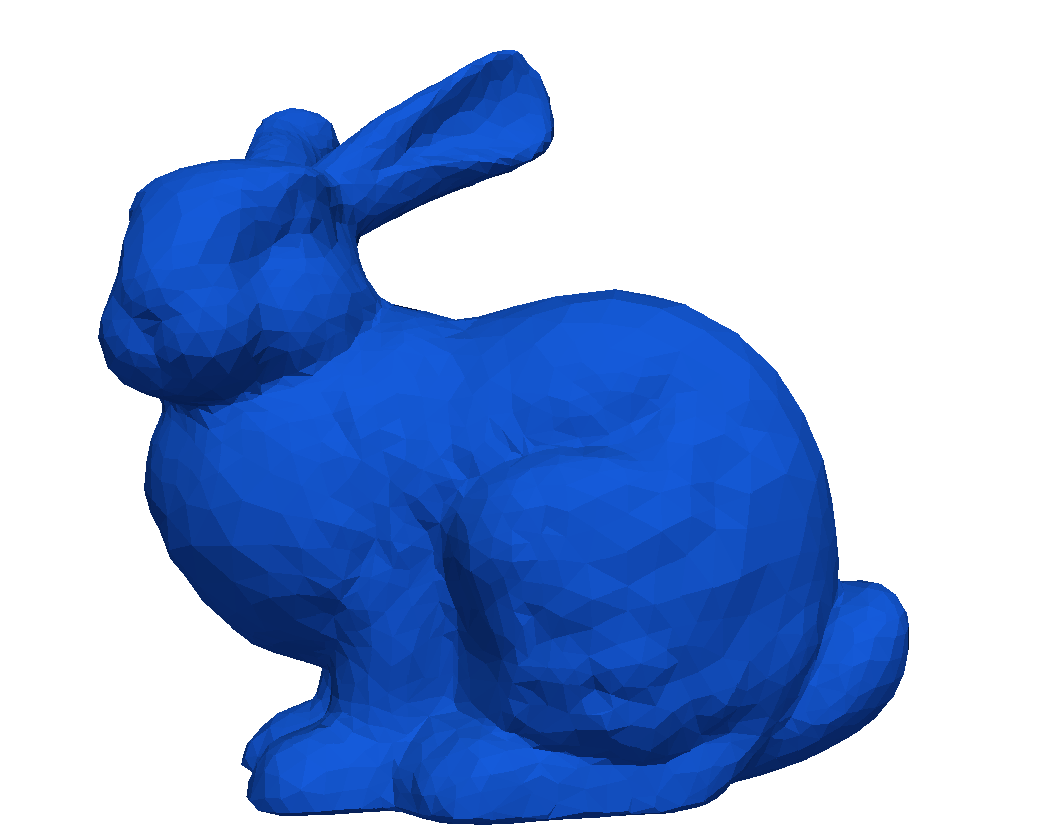
\includegraphics[width=0.5\textwidth]{bunny_initial_front.png}
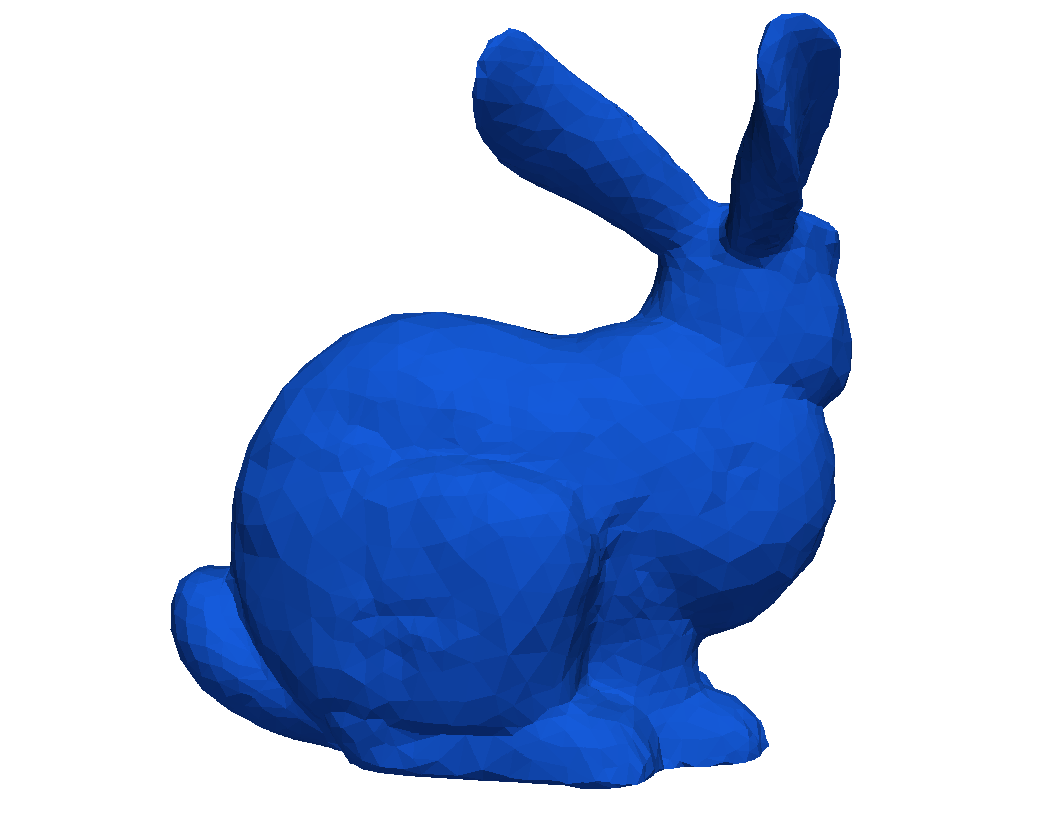
\includegraphics[width=0.5\textwidth]{bunny_initial_back.png}
\caption{Initial state of the bunny.}
\label{fig:bunny_initial}
\end{figure}

In figure \ref{fig:bunny_ear_displacement} and \ref{fig:bunny_gravity} the wireframe model shows the initial state of the bunny. 
Its deformed state is represented by the solid model.
We obtain the deformation as shown in figure \ref{fig:bunny_ear_displacement} if we set the gravity in the parameter file \ref{sec:parameter_file} to $-9.81$
\begin{lstlisting}[breaklines]
  Parameter File -> ElasticityModel -> gravity -> -9.81
\end{lstlisting}
and change the displacement of the tips of the ears in the file \ref{sssec:StationaryElasticityAssemblerDirichletBC3D} as follows:
\lstinputlisting[language=CustomC++]{Code/bunny_ear_displacement.h}

\begin{figure}[htb]
\centering
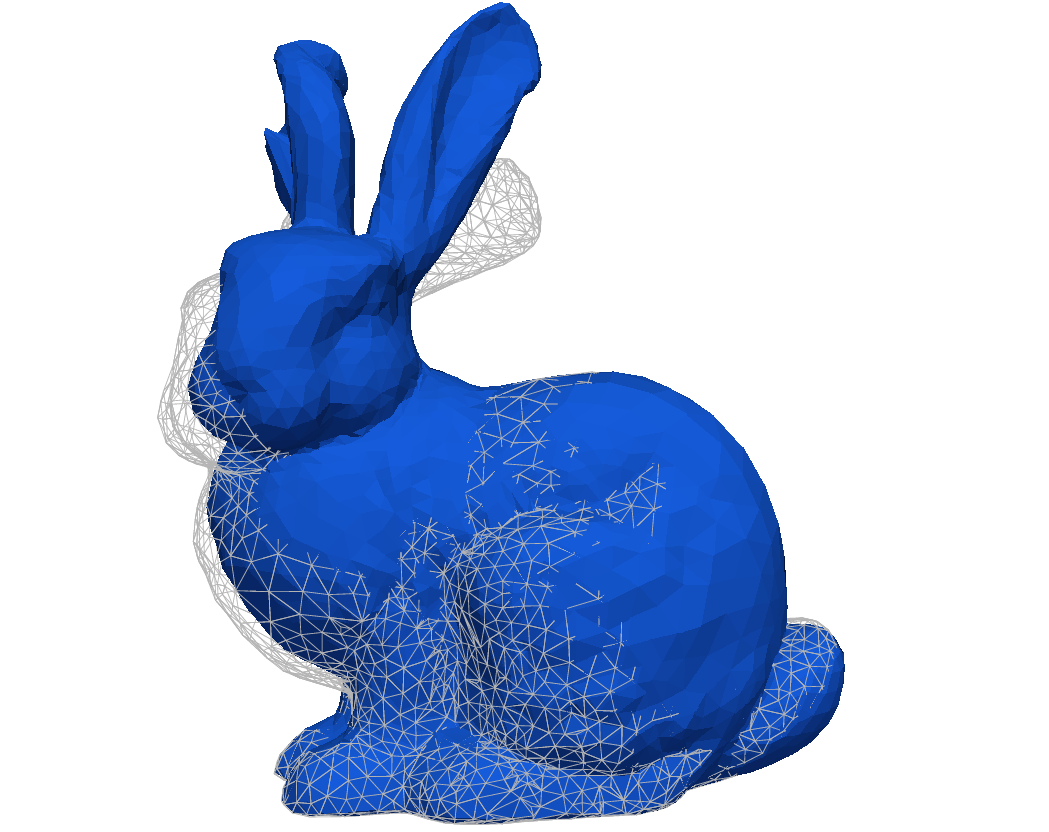
\includegraphics[width=0.5\textwidth]{bunny_ear_displacement_front.png}
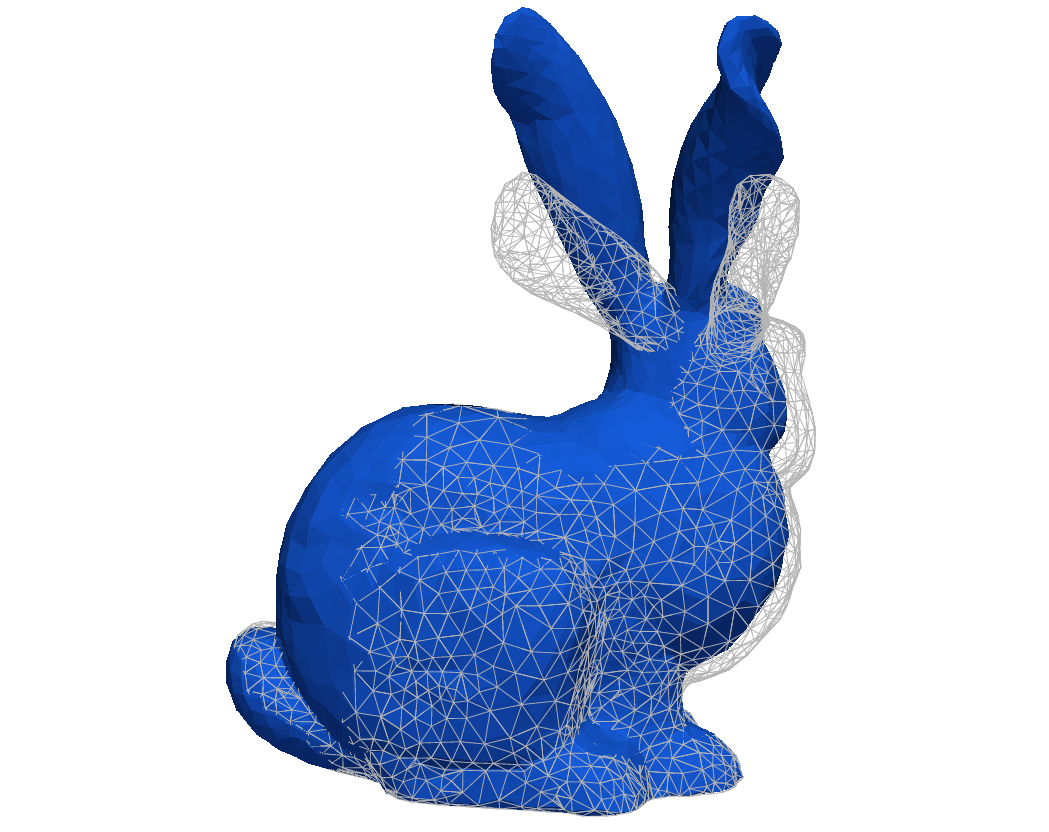
\includegraphics[width=0.5\textwidth]{bunny_ear_displacement_back.png}
\caption{Fixed displacement of the tips of the bunny's ears.}
\label{fig:bunny_ear_displacement}
\end{figure}

Setting the gravity to $-300.00$
\begin{lstlisting}[breaklines]
  Parameter File -> ElasticityModel -> gravity -> -300.00
\end{lstlisting}
and the displacement of the ears as shown in the code below, leads to the deformation displayed in figure \ref{fig:bunny_gravity}.
\lstinputlisting[language=CustomC++]{Code/bunny_gravity.h} 

\begin{figure}[htb]
\centering
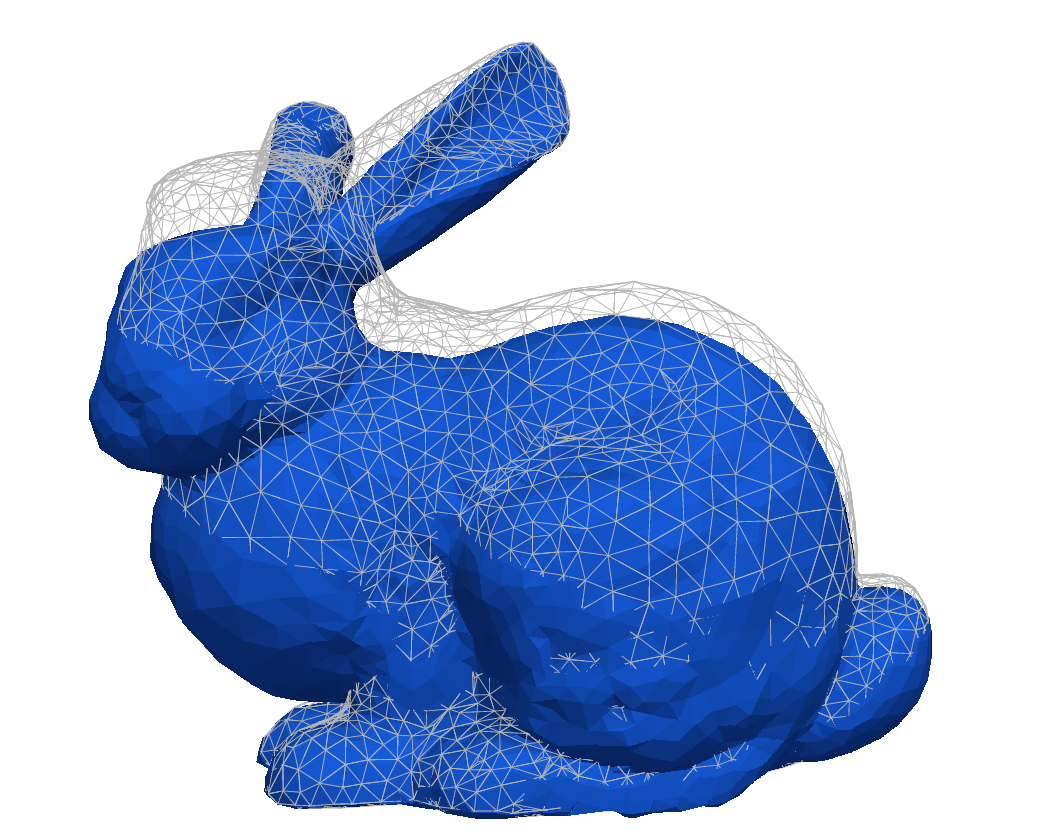
\includegraphics[width=0.5\textwidth]{bunny_gravity_front.png}
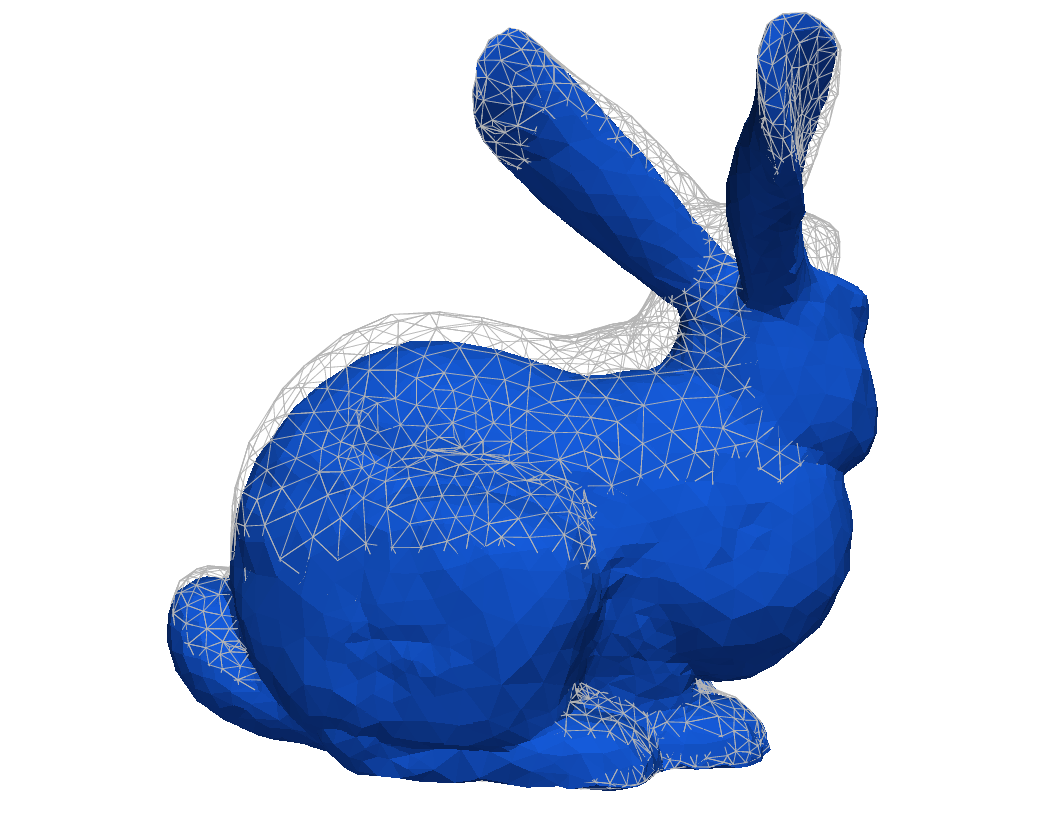
\includegraphics[width=0.5\textwidth]{bunny_gravity_back.png}
\caption{Bunny under the influence of increased gravity.}
\label{fig:bunny_gravity}
\end{figure}


%%%%%% Acknowledgements

\section{Acknowledgements}
\label{sec:acknowledgements}

This work was carried out with the support of the German Research Foundation (DFG) within the project I03 of the Collaborative Research Center SFB/TRR 125 'Cognition-Guided Surgery'.


%%%%%%%%%%%


\newpage
\appendix

\bibliography{tutorials_bib}
\bibliographystyle{unsrt}

\printindex

\end{document}
